\subsection{Casos de Uso}
\label{sec:titSecCasoUso}

Segundo \citeonline{guedes2018uml}, o diagrama de casos de uso "apresenta uma linguagem simples e de fácil compreensão para que os usuários possam ter uma ideia geral de como o sistema irá se comportar". São extremamente úteis para expor aos interessados no projeto, as funcionalidades que compõem a aplicação.

\begin{figure}[H]
    \centering
    \caption{Diagrama de Caso de Uso Geral}
    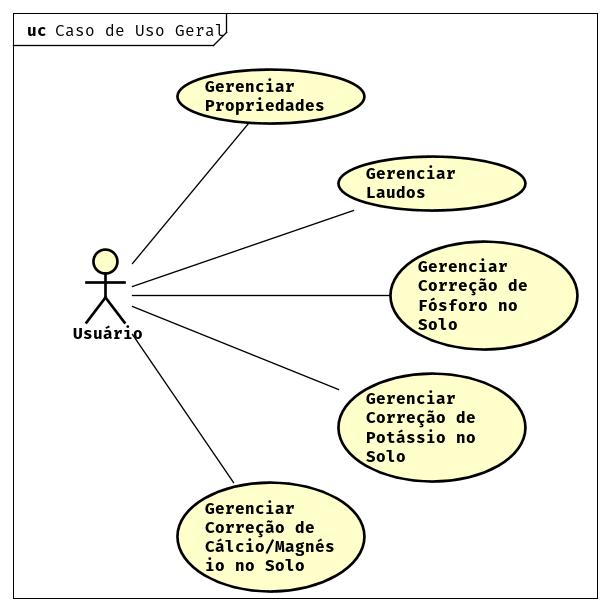
\includegraphics[width=13cm]{dados/figuras/casouso.jpg}
    \label{fig:diagramaCasoUso}
    \fonte{Autoria própria}
\end{figure}

Os casos de uso estão intimamente relacionados aos requisitos funcionais enumerados na \autoref{rf:tabela} e que serão comentados nas subseções abaixo.

\subsubsection{Caso de Uso - Gerenciar propriedades}
\label{sec:titSecCasoUsoPropriedades}

O Caso de Uso "Gerenciar propriedades" está relacionado ao requisito funcional RF001. Um propriedade representa uma área pertencente à um agricultor, como um sítio ou fazenda. Cada propriedade possui uma ou várias partições ou talhões, que será analisada, sendo assim, de suma importância para o funcionamento da aplicação. Como um produtor pode ter várias áreas analisadas em uma propriedades, faz-se necessário a criação de uma entidade no sistema.

\subsubsection{Caso de Uso - Gerenciar laudos}
\label{sec:titSecCasoUsoLaudos}

O caso de uso "Gerenciar laudos" referencia os RF02 a RF06. O laudo técnico do solo representa os indicadores de nutrientes do solo de um determinado talhão. Um talhão pode ser analisado diversas vezes. Por isso é importante que este laudo seja gerenciável como uma entidade na aplicação.

\subsubsection{Caso de Uso - Gerenciar correção de fósforo no solo}
\label{sec:titSecCasoUsoFosforo}

O caso de uso "Gerenciar correção de fósforo no solo" referencia os RF07 a RF09. As variáveis de correção do solo são: fonte de corretivo, eficiência, custo por tonelada. As fontes de corretivo possuem um valor padrão, que o usuário poderá editar no momento da realização do cálculo pois um determinado corretivo pode ser vendido com o mesmo nome mas ter propriedades diferentes. Por isso é necessário tornar gerenciável.

\subsubsection{Caso de Uso - Gerenciar correção de potássio no solo}
\label{sec:titSecCasoUsoPotassio}

O caso de uso "Gerenciar correção de potássio no solo" referencia os RF10 a RF12. Caso a saturação de bases fique além do ideal, é possível alterar o percentual desejado de potássio na CTC. Também deve ser possível o usuário alterar o valor em R\$/ton da fonte de potássio.

\subsubsection{Caso de Uso - Gerenciar correção do cálcio e magnésio no solo}
\label{sec:titSecCasoUsoCalcioMagnesio}

O caso de uso "Gerenciar correção do cálcio e magnésio no solo" referencia os RF13 a RF25. Caso a saturação de bases fique além do necessário, o usuário do sistema poderá corrigir o percentual de cálcio desejado na CTC. Além disso, também deve ser possível o usuário alterar o valor padrão do PRNT do corretivo, bem como o valor em R\$/ton.